\subsubsection{Mô tả thuật toán phát sinh khóa}

Tải tệp \texttt{3.exe} vào công cụ \texttt{OllyDbg}, sau đó sử dụng chức năng \textit{Search for \textrightarrow\ All referenced text strings} để lọc các chuỗi ký tự đáng chú ý. Một trong những chuỗi có thể thu hút sự quan tâm được minh họa như sau:

\begin{center}
    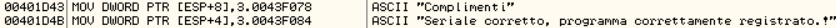
\includegraphics[width=\textwidth]{img/file-3/1.png}
\end{center}

Di chuyển đến dòng mã chứa chuỗi trên, có thể quan sát thấy các lệnh gọi đến hàm \texttt{GetDlgItem}. Đây là một API của Windows, thường được sử dụng trong các ứng dụng giao diện đồ họa (GUI) để lấy \textit{handle} của một control như ô nhập liệu, nút nhấn, v.v.

Vì đây là vị trí có khả năng cao chứa logic xử lý dữ liệu đầu vào, cần đặt các breakpoint tại các lệnh gọi hàm \texttt{GetDlgItem} và \texttt{GetDlgItemTextA} để theo dõi quá trình hoạt động của chương trình. Cụ thể, các địa chỉ đặt breakpoint gồm: \texttt{0x401888}, \texttt{0x4018DC}, \texttt{0x401CBB}, và \texttt{0x401CF7}.

\vspace{0.5em}
Sau khi đặt breakpoint, tiến hành debug và nhập thông tin:

\begin{center}
    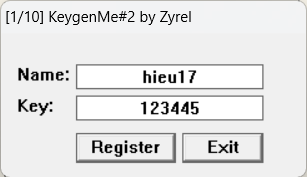
\includegraphics[width=0.5\textwidth]{img/file-3/2.png}
\end{center}

Tại breakpoint đầu tiên, quan sát tại địa chỉ \texttt{0x401898} thấy chương trình gọi API \texttt{GetWindowTextLengthA} để lấy độ dài chuỗi \texttt{Name} và lưu kết quả vào thanh ghi \texttt{EAX}. Ngay sau đó, chương trình so sánh \texttt{EAX} với 4. Nếu \texttt{EAX} $\leq$ 4, luồng thực thi sẽ nhảy xuống địa chỉ \texttt{0x00401FD4}. Điều này cho thấy điều kiện ràng buộc đầu tiên là \textbf{độ dài chuỗi \texttt{Name} phải lớn hơn 4}.

\begin{center}
    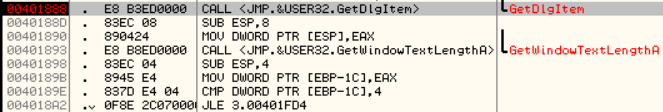
\includegraphics[width=\textwidth]{img/file-3/3.png}
\end{center}

Tại breakpoint thứ hai, quan sát thấy một vòng lặp đang được thực hiện.

\begin{center}
    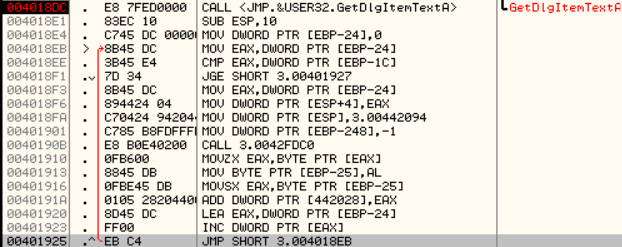
\includegraphics[width=\textwidth]{img/file-3/4.png}
\end{center}

Vòng lặp này tính tổng mã ASCII của các ký tự trong chuỗi \texttt{Name} và lưu kết quà vào địa chỉ \texttt{0x442028}. Với chuỗi ví dụ là \texttt{hieu17}, tổng sẽ là:
\[
\texttt{68 + 69 + 65 + 75 + 31 + 37 = 213}
\]

Quan sát đoạn mã tiếp theo:

\begin{center}
    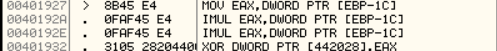
\includegraphics[width=\textwidth]{img/file-3/5.png}
\end{center}

Thực hiện phép toán lấy độ dài chuỗi \texttt{Name} mũ 3 rồi XOR với tổng ASCII vừa tính và lưu lại vào địa chỉ \texttt{0x442028}. Với độ dài là 6, phép toán thực hiện là:
\[
6^3 \;\mathrm{XOR}\; 213 = 2CB
\]

Tiếp tục trace đến địa chỉ \texttt{0x40197D}:

\begin{center}
    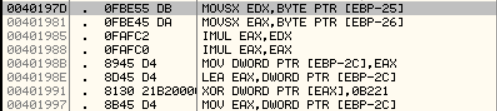
\includegraphics[width=\textwidth]{img/file-3/6.png}
\end{center}

Chương trình lấy mã ASCII của ký tự đầu tiên và ký tự cuối cùng trong chuỗi \texttt{Name}, nhân với nhau, sau đó bình phương kết quả vừa tính. Cuối cùng, kết quả đó được XOR với hằng số \texttt{B221}. Cụ thể:

\[
(68 \times 37)^2 \;\mathrm{XOR}\; B221 = 1F38C61
\]

Tại địa chỉ \texttt{0x4019A4}:

\begin{center}
    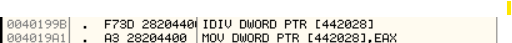
\includegraphics[width=\textwidth]{img/file-3/7.png}
\end{center}

Kết quả từ bước trên sau đó được chia cho giá trị tại vùng nhớ \texttt{0x442028}. Cụ thể: 
\[
    1F38C61 \div 2CB = B2DB
\] 

Tại breakpoint thứ ba, không có thao tác đặc biệt đáng chú ý. Di chuyển đến breakpoint thứ tư:

\begin{center}
    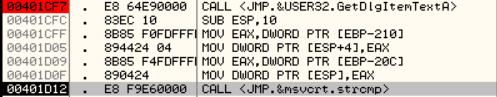
\includegraphics[width=\textwidth]{img/file-3/8.png}
\end{center}

Tại địa chỉ \texttt{0x401D12}, chương trình gọi hàm \texttt{strcmp} để so sánh chuỗi. Quan sát trong cửa sổ thanh ghi, thấy xuất hiện cặp giá trị: \texttt{45787-32738401}.

\begin{center}
    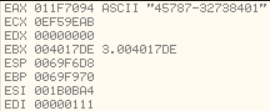
\includegraphics[width=0.5\textwidth]{img/file-3/9.png}
\end{center}

Tiến hành nhập lại trong chương trình \texttt{3.exe} với \texttt{Name} là \texttt{"hieu17"} và \texttt{Serial} là \texttt{"45787-32738401"} thì xuất hiện thông báo chúc mừng. Như vậy, đây chính là serial hợp lệ tương ứng với chuỗi \texttt{Name = "hieu17"}.
Có thể nhận thấy, phần đầu của key là hệ thập phân của \texttt{B2DB} và phần sau là hệ thập phân của \texttt{1F38C61} mà hai kết quả này ta đã tính ở trên.
Từ đây suy ra thuật toán keygen như sau:
\[
S = \sum_{i=1}^{n} \mathrm{ascii}(c_i), n > 4
\]
\[
\text{prefix} = \left\lfloor \dfrac{ \left( \mathrm{ascii}(c_1) \cdot \mathrm{ascii}(c_n) \right)^2 \;\mathrm{XOR}\; 45601 }{ n^3 \;\mathrm{XOR}\; S } \right\rfloor
\]
\[
\text{suffix} = \left( \mathrm{ascii}(c_1) \cdot \mathrm{ascii}(c_n) \right)^2 \;\mathrm{XOR}\; 45601
\]
\[
\text{Key} = \text{"}\texttt{prefix} \text{-} \texttt{suffix}\text{"}
\]

\subsubsection{Chương trình phát sinh khóa}
\begin{lstlisting}[language=Python, caption={Chương trình phát sinh khóa}] 
def keygen3(name: str) -> str:
    if len(name) <= 4:
        return "Name too short"

    ascii_sum = sum(ord(char) for char in name)
    suffix = ((ord(name[0]) * ord(name[-1])) ** 2) ^ 0xB221
    prefix = suffix // ((len(name)**3) ^ ascii_sum)

    return f"{prefix}-{suffix}"
\end{lstlisting}